\documentclass[a4paper]{article}
%%%%%Paquetes%%%%%
\usepackage[T1]{fontenc}
\usepackage[utf8]{inputenc}
\usepackage[spanish]{babel}
\usepackage{amsmath,amssymb,eucal,mathrsfs}
\usepackage[svgnames,X_11names]{xcolor}
\usepackage{colortbl}
\usepackage{Estilos/MiEstilo}
%\usepackage{Estilos/Informe}
\usepackage{amsmath}
\usepackage{times}
\usepackage{color}
\usepackage{listings}
\usepackage{graphicx}
\usepackage{caption}

	\setcounter{tocdepth}{2} %Mostrar solo 3 niveles en el índice
		\makeindex	%índice de palabras
		\title{Teoría de Autómatas y Lenguajes Formales.\\ AFD para multiplos de 3. }
		\author{Luis José Quintana Bolaño}
		\date{\today}

\begin{document}
		\maketitle
		\begin{abstract}
		    Encontrar un AFD, que llamaremos A, que reconozca números binarios múltiplos de 3. Es decir:
		    $$L(A)=\{0,11_{(\text{el 3})},110_{(\text{el 6})},1001_{(\text{el 9})},...\}$$
  		\end{abstract}

  		\section{Grafo de transiciones}
  			\begin{figure}[!h]
  			\centering
  			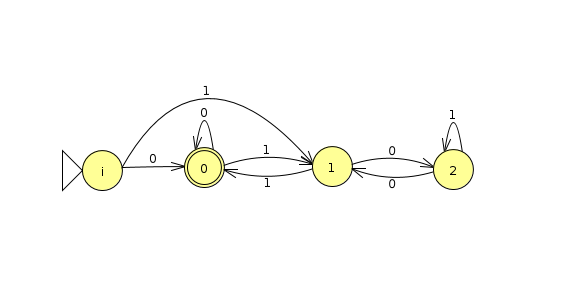
\includegraphics[trim= 30 100 50 80,clip]{DFA.png}
  			\caption{Grafo de transiciones}
  			\end{figure}
  		\section{Tabla de transiciones}
  			\begin{figure}[!h]
  			\centering
  			\begin{tabular}{r|c|c|} 
  				   & 0 & 1 \\ \hline
  				i  & 0 & 1 \\ \hline
			    *0  & 0 & 1 \\ \hline
			    1  & 2 & 0 \\ \hline
			    2  & 1 & 2 \\ \hline
  		    \end{tabular} \\
  		    \caption{Tabla de transiciones}
  		    \end{figure}
  		\section{Corrección y Completitud}
  		Demostración por inducción múltiple.

  		\begin{equation}
  			\text{Hipótesis de inducción} \equiv \left\{
  			\begin{array}{rcl}
  				\delta(i, x) = 0 &\Rightarrow& x\bmod3=0 \\
  				\delta(i, x) = 1 &\Rightarrow& x\bmod3=1 \\
  				\delta(i, x) = 2 &\Rightarrow& x\bmod3=2 \\
  				\delta(i, x) = i &\Rightarrow& x\equiv\epsilon
  				\end{array}\right.
  			\label{eq:hi}
  		\end{equation}

  		Caso base: $|w|=\epsilon$

  		Asumimos que la hipótesis (\ref{eq:hi}) es cierta para cadenas de longitud inferior a la de $w$, siendo $|w|\geq1$. Como $w$ no es vacía, podemos considerar $w=xa$, donde $a$ es el último miembro de $w$ y $x$ es la cadena que la precede, por tanto la hipótesis de inducción (\ref{eq:hi}) se cumple para $x$.

  		Procedemos a demostrar su corrección para $w=xa$:
  		\begin{enumerate}
  		\item Si $\delta(i, w) = 0$, $a$ puede ser $0$ o $1$:
  			\begin{enumerate}
  			\item Si $a=0$, de acuerdo a la tabla de transiciones:
  				\begin{enumerate}
  				\item $\delta(i, x) = 0$ y, por h.i., $x\bmod3=0$, $x0 = x*2$, luego $x*2\bmod3=0$ es cierto.
  				\item $\delta(i, x) = i$ y, por h.i., $x\equiv\epsilon \rightarrow x0 = 0$, luego $0\bmod3=0$ es cierto.
  				\end{enumerate}
  			\item Si $a=1$, de acuerdo a la tabla de transiciones $\delta(i, x) = 1$ y, por h.i., $x\bmod3=1 \rightarrow x=n*3+1$, $x1=2x+1 \rightarrow x1=3n+1$, luego $3n+1\bmod3=1$ es cierto.
  			\end{enumerate}
  		\item Si $\delta(i, w) = 1$, $a$ puede ser $0$ o $1$:
  			\begin{enumerate}
  			\item Si $a=0$, de acuerdo con la tabla de transiciones $\delta(i, x) = 2$ y, por h.i., $x\bmod3=2 \rightarrow x=n*3+2$, $x0=x*2 \rightarrow x0=n6+4$, luego $x0\bmod3=1$ es cierto.
  			\item Si $a=1$, de acuerdo con la tabla de transiciones:
  				\begin{enumerate}
  				\item $\delta(i, x) = 0$ y, por h.i., $x\bmod3=0$, $x0 = x*2$, luego $x0\bmod3=0$ es cierto.
  				\item $\delta(i, x) = i$ y, por h.i., $x\equiv\epsilon \rightarrow x0 = 0$, luego $0\bmod3=0$ es cierto.
  				\end{enumerate}
  			\end{enumerate}
  		\item Si $\delta(i, w) = 2$, $a$ puede ser $0$ o $1$:
  			\begin{enumerate}
  			\item Si $a=0$, de acuerdo a la tabla de transiciones $\delta(i, x) = 1$ y, por h.i., $x\bmod3=1 \rightarrow x=n*3+1$, $x0=x*2 \rightarrow x0=n*6+2$, luego $x0\bmod3=2$ es cierto.
  			\item Si $a=1$, de acuerdo a la tabla de transiciones $\delta(i, x) = 2$ y, por h.i., $x\bmod3=2 \rightarrow x=n*3+2$, $x1=x*2+1 \rightarrow x0=n*6+5$, luego $x1\bmod3=2$ es cierto.
  			\end{enumerate}
  		\end{enumerate}

  		La hipótesis de inducción (\ref{eq:hi}) se cumple para todos los casos, por lo que el AFD es correcto y completo.

  		\section{Implementación en C del AFD}
  		\subsection{Método de los cases}
  		\lstinputlisting[language=C]{cases.c}
  		\subsection{Método de la tabla}
  		\lstinputlisting[language=C]{table.c}
  		
\end{document}
